This appendix provides a comprehensive presentation of the transmission opportunity (txops) files collected during the experiments described in Chapter \ref{chap:measurements}. These files capture Orange commercial 4G network characteristics and are available as Open Data \footnote{\url{https://cloud-gaming-traces.lhs.loria.fr/data.html}}. For each of the six (06) txops files, two figures are included:
\begin{itemize}
    \item \textbf{The Cumulative Distribution Function} illustrating the distribution of the number of packets per txops.
    \item \textbf{The throughput analysis}, which highlights the data rate behavior across the network conditions.
\end{itemize}


By visualizing these metrics, the appendix aims to offer insights into the network conditions observed during the experiments, serving as a valuable resource for understanding the basis of the datasets used throughout this thesis. Each section corresponds to one txops file, presenting both figures side by side for clarity and easy comparison. 


% \section{Txops File E}

\begin{figure*}[!ht]
  \centering
  \begin{tabular}{ c @{\hspace{0pt}} c}
  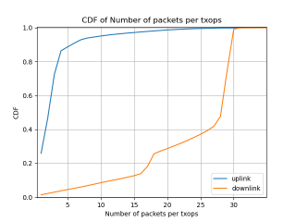
\includegraphics[width=0.4\textwidth]{imgs/appendix_2/E_cdf.png}
    &
  %\medskip
    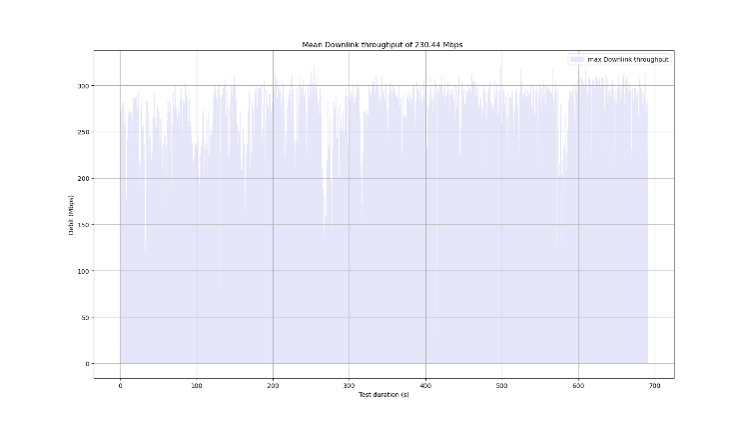
\includegraphics[width=0.5\textwidth]{imgs/appendix_2/E_throughput.png}\\
     \small \textbf{(a) CDF of the number of packets per txops} &
    \small \textbf{(b) Downlink throughput capacity}  \\
  \end{tabular}
  \medskip
  \caption{Txops File E.}
  \label{fig:app_2:txops_E}
\end{figure*}

% \section{Txops File D}

\begin{figure*}[!ht]
  \centering
  \begin{tabular}{ c @{\hspace{0pt}} c}
  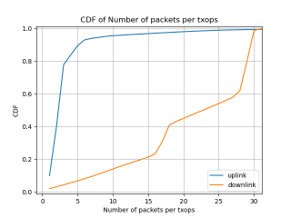
\includegraphics[width=0.4\textwidth]{imgs/appendix_2/D_cdf.png}
    &
  %\medskip
    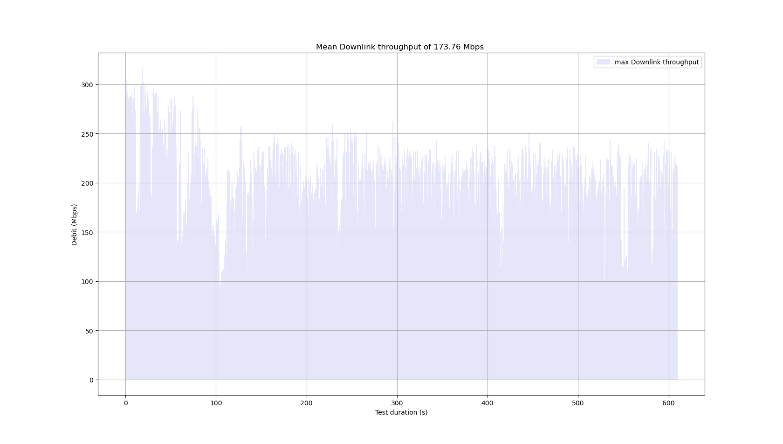
\includegraphics[width=0.5\textwidth]{imgs/appendix_2/D_throughput.png}\\
     \small \textbf{(a) CDF of the number of packets per txops} &
    \small \textbf{(b) Downlink throughput capacity}  \\
  \end{tabular}
  \medskip
  \caption{Txops File D.}
  \label{fig:app_2:txops_D}
\end{figure*}

% \section{Txops File C}

\begin{figure*}[!ht]
  \centering
  \begin{tabular}{ c @{\hspace{0pt}} c}
  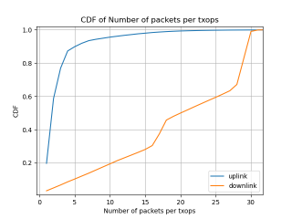
\includegraphics[width=0.4\textwidth]{imgs/appendix_2/C_cdf.png}
    &
  %\medskip
    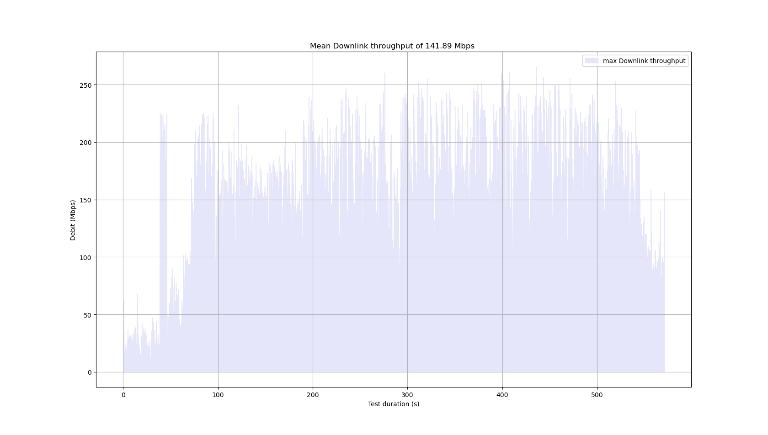
\includegraphics[width=0.5\textwidth]{imgs/appendix_2/C_throughput.png}\\
     \small \textbf{(a) CDF of the number of packets per txops} &
    \small \textbf{(b) Downlink throughput capacity}  \\
  \end{tabular}
  \medskip
  \caption{Txops File C.}
  \label{fig:app_2:txops_C}
\end{figure*}

% \section{Txops File B}

\begin{figure*}[!ht]
  \centering
  \begin{tabular}{ c @{\hspace{0pt}} c}
  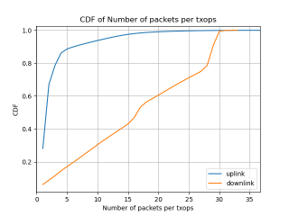
\includegraphics[width=0.4\textwidth]{imgs/appendix_2/B_cdf.png}
    &
  %\medskip
    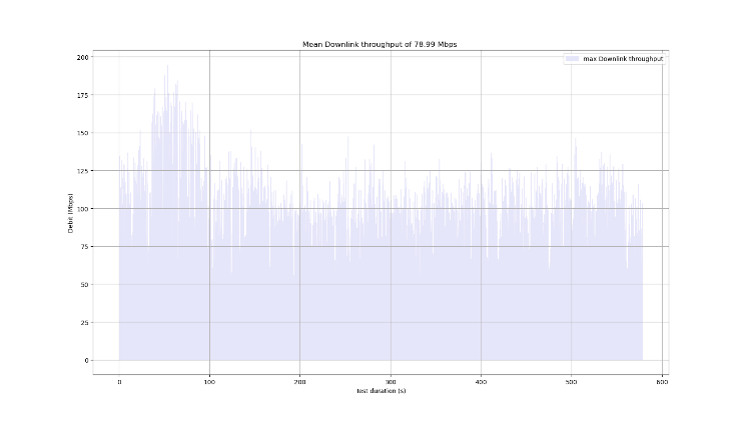
\includegraphics[width=0.5\textwidth]{imgs/appendix_2/B_throughput.png}\\
     \small \textbf{(a) CDF of the number of packets per txops} &
    \small \textbf{(b) Downlink throughput capacity}  \\
  \end{tabular}
  \medskip
  \caption{Txops File B.}
  \label{fig:app_2:txops_B}
\end{figure*}

% \section{Txops File A}

\begin{figure*}[!ht]
  \centering
  \begin{tabular}{ c @{\hspace{0pt}} c}
  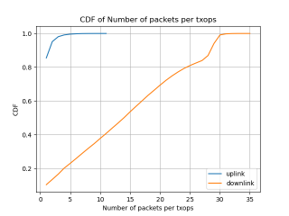
\includegraphics[width=0.4\textwidth]{imgs/appendix_2/A_cdf.png}
    &
  %\medskip
    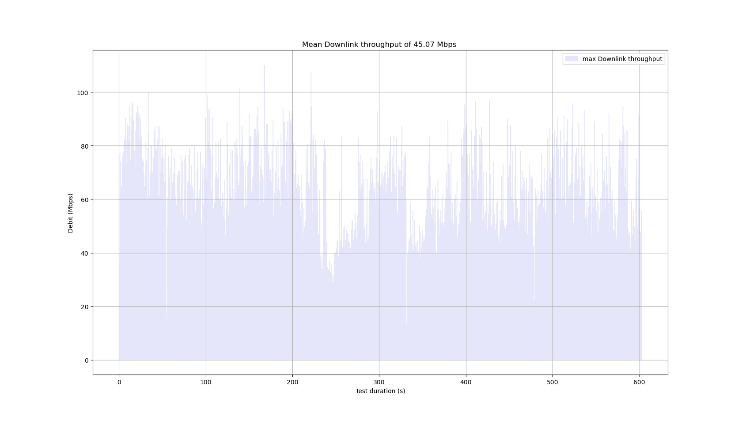
\includegraphics[width=0.5\textwidth]{imgs/appendix_2/A_throughput.png}\\
     \small \textbf{(a) CDF of the number of packets per txops} &
    \small \textbf{(b) Downlink throughput capacity}  \\
  \end{tabular}
  \medskip
  \caption{Txops File A.}
  \label{fig:app_2:txops_A}
\end{figure*}


% \section{Txops File Highway}

\begin{figure*}[!ht]
  \centering
  \begin{tabular}{ c @{\hspace{0pt}} c}
  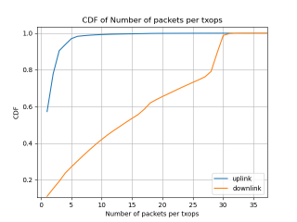
\includegraphics[width=0.4\textwidth]{imgs/appendix_2/highway_cdf.png}
    &
  %\medskip
    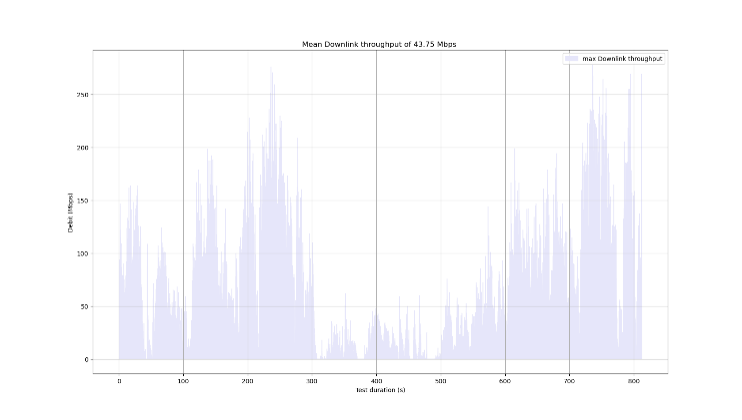
\includegraphics[width=0.5\textwidth]{imgs/appendix_2/highway_throughput.png}\\
     \small \textbf{(a) CDF of the number of packets per txops} &
    \small \textbf{(b) Downlink throughput capacity}  \\
  \end{tabular}
  \medskip
  \caption{Txops File Highway.}
  \label{fig:app_2:txops_highway}
\end{figure*}
